\documentclass[
\pagestyle{fancy}
\setmarginsrb{20mm}{0mm}{20mm}{25mm}{12mm}{11mm}{0mm}{11mm}
\lhead{MA4128} \rhead{Mr. Kevin O'Brien}
\chead{Advanced Data Modelling}
%\input{tcilatex}


\begin{document}



\section{Cluster Analysis: Background to K-Means Clustering}
\noindent \textbf{Objective:} create clusters of items, individuals or objects that have similarity with the others in the cluster but with differences between clusters.  
% Document prepared by Robert L. Andrews, April 2005 & revised, April 2011

\begin{itemize}
	\item The items, individuals or objects being placed into clusters will be referred to as cases.  The degree of similarity or dissimilarity may be determined from the recorded values for one or multiple characteristics for the cases. There are no dependent variables for cluster analysis.  
\item Clustering procedures require that similarity be quantified.  One quantitative measure for interval scale data is the distance between cases.  Euclidean Distance measures the length of a straight line between two cases.  The numeric value of the distance between cases depends on the measurement scale.  
\item If the measurements are recorded using different measurement scales then one should use a \textbf{transformation} to assure similar variability of measurements for all characteristics being used to create the clusters.\textit{(We will revert to transforming data later in the course.) }
%(see Transform Values section below tell how this can be done in SPSS Hierarchical Cluster Analysis, otherwise this needs to be done prior to the analysis, for example, when using SPSS K-Means Cluster Analysis).  
\item Other measures may be used to create a dissimilarity or distance matrix that can be used as the basis for creating clusters. % (see Measures for Interval Data section under Hierarchical Cluster Analysis).  
	
\item A key issue in obtaining a set of clusters is the determination of the number of clusters.  Hierarchical procedures provide information that allows the analyst to decide on the number of clusters based on the output. 
\item  This is often done by examining tabular or graphical output to identify the gaps that define logical clusters.  
	\item Hierarchical clustering requires a distance or similarity matrix between all pairs of cases. That's an extremely large matrix if you have tens of thousands of cases in your data file.
\end{itemize}
\section{K-means Clustering}
\begin{itemize}
\item A clustering method that doesn't require computation of all possible distances is k-means clustering. It differs from hierarchical clustering in several ways. You have to know in advance the number of clusters you want. You can't get solutions for a range of cluster numbers unless you rerun the analysis for each different number of clusters.

\item The algorithm repeatedly reassigns cases to clusters, so the same case can move from cluster to cluster during the analysis. In agglomerative hierarchical clustering, on the other hand, cases are added only to existing clusters. They are forever captive in their cluster, with a widening circle of ``neighbours".

\item \textbf{Important:} The SPSS K-Means Cluster Analysis procedure requires that the number of clusters be specified in advance to run the analysis. 
\item  The K-Means procedure is applicable for data sets with a large number of cases while the hierarchical procedure may be preferred when there are a limited number of cases.


	\item The algorithm is called \textbf{k-means}, where \textbf{k} is the number of clusters you want, since a case is assigned to the cluster for which its distance to the cluster mean is the smallest.
	
	\item The k-means algorithm follows an entirely different concept than the hierarchical methods
	discussed before. This algorithm is not based on distance measures such as
	Euclidean distance or city-block distance, but uses some sort of group linkage metric, such as  \textbf{\textit{within-cluster variation}}, as a measure to form homogenuous clusters. Specifically, this procedure aims at segmenting
	the data in such away that the within-cluster variation is minimized. Consequently,we
	do not need to decide on a distance measure in the first step of the analysis.
	
	\item The action in the algorithm centers around finding the k-means. You start out with an initial set of means and classify cases based on their distances to the centers.
	
	\item Next, you compute the cluster means again, using the cases that are assigned to the cluster; then, you reclassify all cases based on the new set of means. You keep repeating this step until cluster means don't change much between successive steps.
	
	\item Finally, you calculate the means of the clusters once again and assign the cases to their permanent clusters.
\end{itemize}

\subsection*{Assumptions}
\begin{itemize}
	\item  Distances are computed using simple Euclidean distance. If you want to use another distance or similarity measure, use the Hierarchical Cluster Analysis procedure. 
	\begin{itemize}
		\item[$\ast$] Scaling of variables is an important consideration--if your variables are measured on different scales (for example, one variable is expressed in dollars and another is expressed in years), your results may be misleading.
	\end{itemize}
	\item  In such cases, you should consider standardizing your variables before you perform the k-means cluster analysis \\ (\textit{SPSS: this can be done in the Descriptives procedure}). The procedure assumes that you have selected the appropriate number of clusters and that you have included all relevant variables. 
	\item If you have chosen an inappropriate number of clusters or omitted important variables, your results may be misleading.
\end{itemize}


\subsection*{Case and Initial Cluster Center Order} 
\begin{itemize}
	\item The default algorithm for choosing initial cluster centers is not invariant to case ordering. The Use running means option on the Iterate dialog box makes the resulting solution potentially dependent upon case order regardless of how initial cluster centers are chosen. 
	\item If you are using either of these methods, you may want to obtain several different solutions with cases sorted in different random orders to verify the stability of a given solution. \item Specifying initial cluster centers and not using the Use running means option will avoid issues related to case order. However, ordering of the initial cluster centers may affect the solution, if there are tied distances from cases to cluster centers. Comparing results from analyses with different permutations of the initial center values may be used to assess the stability of a given solution.
	\end{itemize}
%------------------------------------------------------------------%
\subsection{Initial Cluster Centres}
\begin{itemize}
	\item The first step in k-means clustering is finding the k centres. This is done iteratively. You start with an initial set of centres and then modify them until the change between two iterations is small enough.
	
\item If you have good guesses for the centres, you can use those
	as initial starting points; otherwise, you can let SPSS find k cases that are well separated and use these values as initial cluster centers. (i.e. The clustering process starts by randomly assigning objects to a number of
	clusters).
\item K-means clustering is very sensitive to outliers, since they will usually be selected as initial cluster centers. This will result in outliers forming clusters with small numbers of cases. Before you start a cluster analysis, screen the data for outliers and remove them from the initial analysis. The solution may also depend on the order of the cases in the data.
	
\item After the initial cluster centers have been selected, each case is assigned to the closest
	cluster, based on its distance from the cluster centers. After all of the cases have been
	assigned to clusters, the cluster centers are recomputed, based on all of the cases in the
	cluster.
	
\item The cases are then successively reassigned to other clusters to minimize the within-cluster variation, which is basically the (squared) distance from each observation to the center of the associated cluster. If the reallocation of an case to another cluster decreases the within-cluster variation, this case is reassigned
	to that cluster.
	
\item Case assignment is done again, using these updated cluster centers. You keep
	assigning cases and recomputing the cluster centers until no cluster center changes
	appreciably or the maximum number of iterations (10 by default) is reached.
\end{itemize}





\newpage
\subsection{Demonstration of K-Means}

\begin{itemize}
\item In this example, two cluster centers are randomly
initiated, which CC1 (first cluster) and CC2 (second cluster).
\begin{figure}[h!]
	\begin{center}
		% Requires \usepackage{graphicx}
		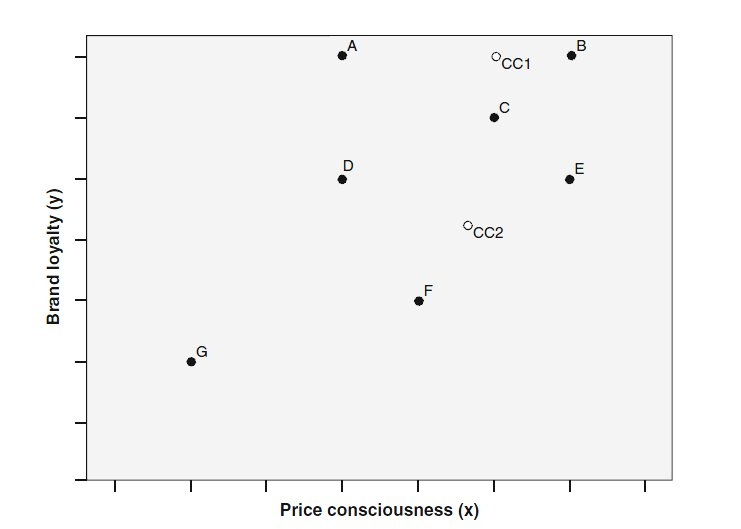
\includegraphics[scale=0.4]{images/kmeans1.jpg}\\
	\end{center}
\end{figure}
\begin{figure}[h!]
	\begin{center}
		% Requires \usepackage{graphicx}
		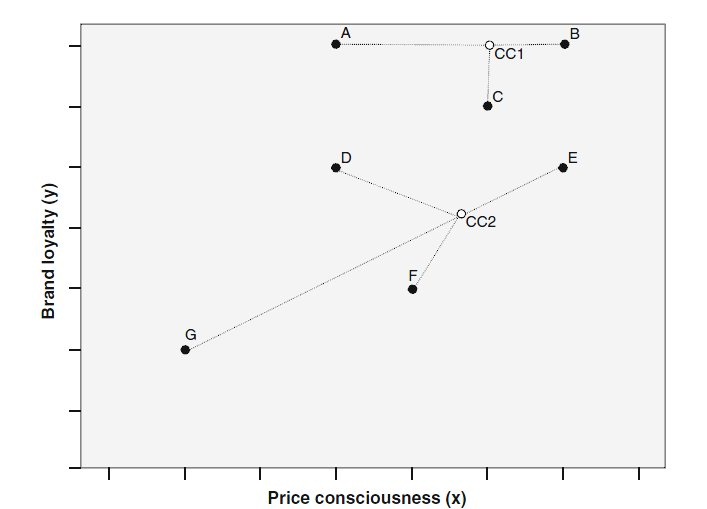
\includegraphics[scale=0.4]{images/kmeans2.jpg}\\
	\end{center}
\end{figure}
\item Euclidean distances are computed from the cluster
centers to every single object. Each object is then assigned to the cluster center with
the shortest distance to it.

\item In this example, objects A, B, and C are
assigned to the first cluster, whereas objects D, E, F, and G are assigned to the
second. We now have our initial partitioning of the objects into two clusters.
\item Based on this initial partition, each cluster’s geometric center (i.e., its centroid)
is computed (third step). This is done by computing the mean values of the objects
contained in the cluster (e.g., A, B, C in the first cluster) regarding each of the variables
(in this example: price consciousness and brand loyalty).
\begin{figure}[h!]
	\begin{center}
		% Requires \usepackage{graphicx}
		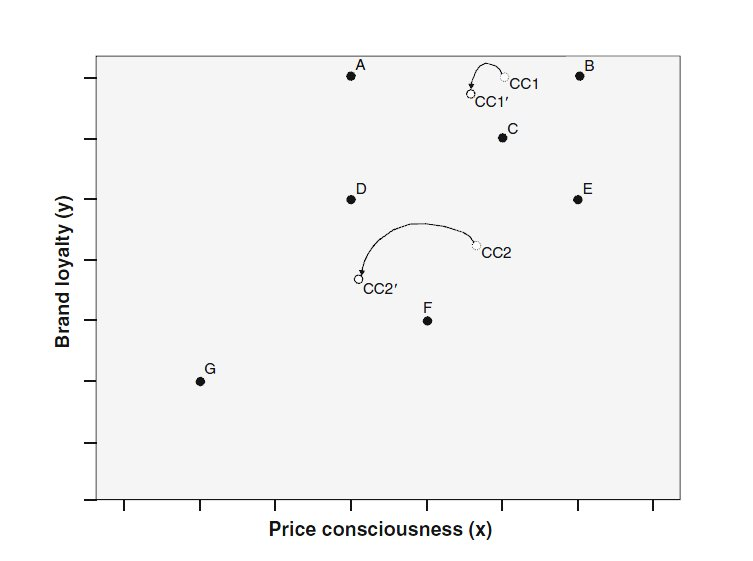
\includegraphics[scale=0.4]{images/kmeans3.jpg}\\
	\end{center}
\end{figure}
\begin{figure}[h!]
	\begin{center}
		% Requires \usepackage{graphicx}
		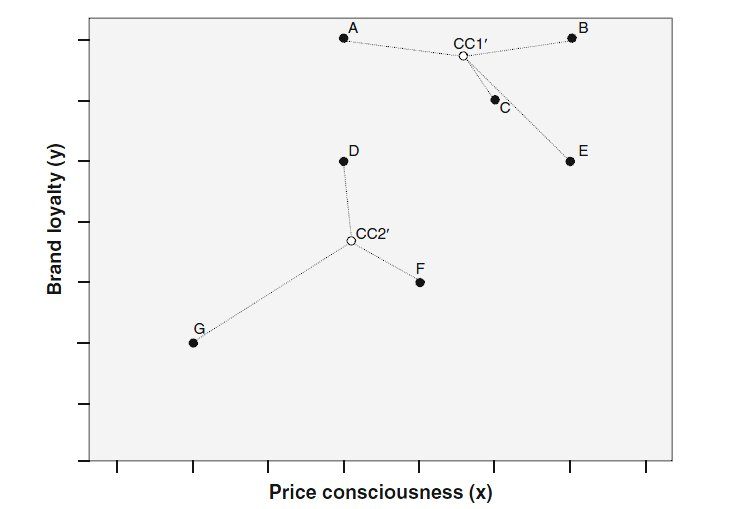
\includegraphics[scale=0.4]{images/kmeans4.jpg}\\
	\end{center}
\end{figure}
\item Both clusters’ centers now shift into new positions (CC1’ for the first and CC2’ for the second cluster).
In the fourth step, the distances from each object to the newly located cluster
centers are computed and objects are again assigned to a certain cluster on the basis
of their minimum distance to other cluster centers (CC1’ and CC2’).

\item Since the cluster centers’ position changed with respect to the initial situation in the first step,
this could lead to a different cluster solution. This is also true of our example, as
object E is now – unlike in the initial partition – closer to the first cluster center
(CC1’) than to the second (CC2’). Consequently, this object is now assigned to the
first cluster.
\item The k-means procedure now repeats the third step and
re-computes the cluster centers of the newly formed clusters, and so on.
\item (\textbf{Important}) In other words, steps 3 and 4 are repeated until a predetermined number of iterations are
reached, or convergence is achieved (i.e., there is no change in the cluster affiliations).
\end{itemize}
\subsection{Performance of K-Means Clustering}
\begin{itemize}
\item Generally, k-means is superior to hierarchical methods as it is less affected by
outliers and the presence of irrelevant clustering variables. Furthermore, k-means
can be applied to very large data sets, as the procedure is less computationally
demanding than hierarchical methods. 
\item In fact, we suggest definitely using k-means
for sample sizes above 500, especially if many clustering variables are used. From
a strictly statistical viewpoint, k-means should only be used on interval or ratio-scaled
data as the procedure relies on Euclidean distances. 
\item However, the procedure is
routinely used on ordinal data as well, even though there might be some distortions.

\item One problem associated with the application of k-means relates to the fact that
the researcher has to pre-specify the number of clusters to retain from the data. This
makes k-means less attractive to some and still hinders its routine application in
practice.
\end{itemize}

% Cluster analysis can be an effective tool to identify extreme data values in a multivariate data set.  Extreme points will be a cluster by themselves while the vast majority of the other points are in one or more well populated clusters.  
% When performing hierarchical cluster analysis one can cluster cases or variables in SPSS by selecting either cases or variables in the initial menu.  The default is cases since it is probably done more than clustering variables but clustering variables may be desirable in certain situations.  

%%%%%%%%%%%%%%%%%%%%%%%%%%%%%%%%%%%%%%%%%%%%%%%%%%%%%%%%%%%%%%%%%%%%%%%%%%%%%%%%%%%%%

\subsection*{K-Means Cluster Analysis}
\begin{itemize}
	\item This procedure attempts to identify relatively homogeneous groups of cases based on selected characteristics, using an algorithm that can handle large numbers of cases.
	\item However, the algorithm requires you to specify the number of clusters. You can specify initial cluster centers if you know this information. \item You can select one of two methods for classifying cases, either updating cluster centers iteratively or classifying only. You can save \texttt{cluster membership}, \texttt{distance information}, and \texttt{final cluster centers}. 
	\item Optionally, you can specify a variable whose values are used to label casewise output. You can also request analysis of variance $F$ statistics.
	\item  While these statistics are opportunistic (the procedure tries to form groups that do differ), the relative size of the statistics provides information about each variable's contribution to the separation of the groups.
	
%	\item Statistics. Complete solution: initial cluster centers, ANOVA table.  Each case: cluster information, distance from cluster center.
\end{itemize}




\subsection*{Implementation}
To Obtain a K-Means Cluster Analysis
From the menus choose:
\begin{verbatim}
Analyze  >  Classify  >  K-Means Cluster...    
\end{verbatim}

\begin{itemize}
\item 	Select the variables to be used in the cluster analysis. 
\item 	Specify the number of clusters. The number of clusters must be at least two and must not be greater than the number of cases in the data file.
\item 	Select either Iterate and classify or Classify only.
\end{itemize}
\end{document}



 
 \newpage
\section*{Clustering Procedures: }
% (Descriptions below originally copied from SPSS13.0 Help & I have made % slight additions.)



\section{Cluster Analysis}


Cluster analysis can be an effective tool to identify extreme data values in a multivariate data set.  Extreme points will be a cluster by themselves while the vast majority of the other points are in one or more well populated clusters.  

When performing hierarchical cluster analysis one can cluster cases or variables in SPSS by selecting either cases or variables in the initial menu.  The default is cases since it is probably done more than clustering variables but clustering variables may be desirable in certain situations.  

\newpage
In these methods the desired number of clusters is specified in advance and the `best' solution
is chosen. The steps in such a method are as follows:
\begin{itemize}
	\item[1] Choose initial cluster centres (essentially this is a set of observations that are far apart
	— each subject forms a cluster of one and its centre is the value of the variables for
	that subject).
	\item[2] Assign each subject to its `nearest' cluster, defined in terms of the distance to the
	centroid.
	\item[3] Find the centroids of the clusters that have been formed
	\item[4] Re-calculate the distance from each subject to each centroid and move observations that
	are not in the cluster that they are closest to.
	\item[5] Continue until the centroids remain relatively stable.
\end{itemize}

\end{document}



